\documentclass{exam}
\usepackage{main}
\qformatExam{}

\title{Contrôle : Généralités sur les fonctions.}
\author{Quentin Canu}
\date{8 Janvier 2023}

\begin{document}
\maketitle
\begin{itemize}
\item Une présentation soignée est de rigueur, et sera notée sur $2$.
\item Tout effort de recherche, même s'il n'aboutit pas, sera valorisé.
\item Toute copie est interdite et sera sanctionnée d'une note de $0$.
\item La calculatrice est interdite.
\end{itemize}
\vspace{0.5cm}
\begin{questions}
\titledquestion{Vrai ou Faux ?}[4]
Soit $f$ est une fonction à valeurs réelles. Les propositions suivantes sont-elles vraies ou fausses ? Il n'est pas nécessaire de justifier les réponses dans cet exercice.
\begin{parts}
\part Si $f(0) = 4$, alors l'image de $0$ par $f$ est $4$.
\part Si $f(-1) = 3$, alors un antécédent de $-1$ par $f$ est $3$
\part Soit $\mathcal{C}_f$ la courbe représentative de $f$ : c'est l'ensemble des points de coordonnées $(x;y)$ vérifiant $f(y)=x$.
\part Le plus grand ensemble de définition de $f$ possible est $\R$. 
\end{parts}
\vspace{0.5cm}
\titledquestion{Equations du premier degré}[4]
Résoudre les équations suivantes dans $\R$ :
\begin{parts}
\part $8x + 2 = 4$
\part $3 - 14t = 5$
\part $28y = 7y + 2$
\part $51a + 12 = 36a - 73$
\end{parts}
\vspace{0.5cm}
\titledquestion{Voyages en voiture}[5]
Trois voitures, $A$, $B$ et $C$ montent au sommet d'une montagne sur la même route de $50$ km. On note $x$ la distance parcourue le long de cette route en kilomètres, et $a(x), b(x)$ et $c(x)$ la vitesse des voitures (en kilomètres par heure) au $x$-ieme kilomètre. On représente ci-dessous la courbe représentative de ces fonctions.
\begin{center}
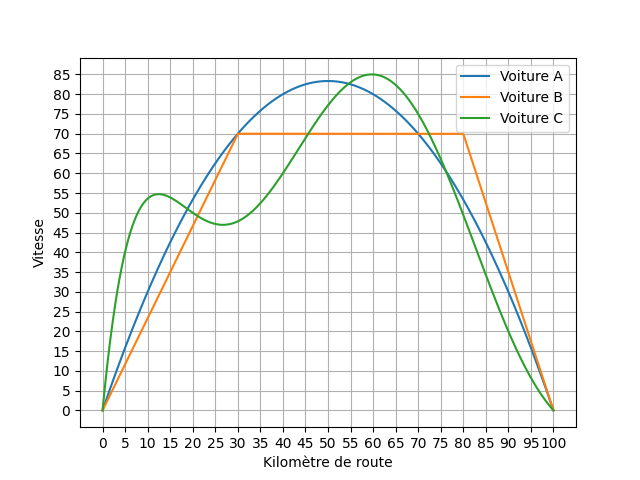
\includegraphics{Route.png}
\end{center}
\begin{parts}
\part Pourquoi $a(0)$, $b(0)$ et $c(0)$ sont-ils tous les trois égaux à $0$ ? Même question pour $a(100)$, $b(100)$ et $c(100)$ ?
\part Donner la vitesse de la voiture $A$ et de la voiture $B$ au kilomètre $30$.
\part Donner sous forme d'intervalle la portion de route sur laquelle la voiture $B$ a été la plus rapide des trois voitures. On utlisera la précision permise par le repère.
\part La route est limitée à $80$ kilomètres par heures.
\begin{subparts}
\subpart Quelles voitures ont enfreint cette limitation ?
\subpart Il y a un radar de vitesse au kilomètre $65$ sur la route. Une des voitures a-t-elle été flashée ? Si oui, laquelle ?
\end{subparts}
\end{parts}

\vspace{0.5cm}
\titledquestion{Comparaison d'aires}[5] On considère une carré $ABCD$ de côté $3$ ainsi qu'un point mobile $M$ sur le segment $[DA]$. On pose alors $E$ sur le segment $[CD]$ et $G$ sur le segment $[BC]$ tel que
\begin{equation*}
DE = DM = CG\,.
\end{equation*}
Enfin, on pose le point $F$ tel que le quadrilatère $DMFE$ soit un carré. Voici ci-dessous une figure pour illustrer.
\begin{center}
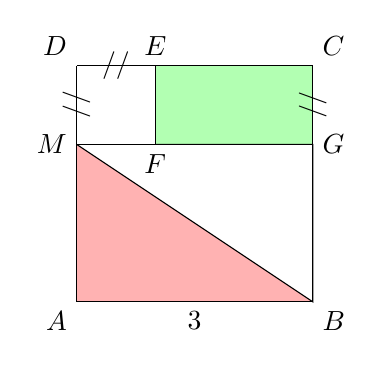
\begin{tikzpicture}
\coordinate (A) at (0,0);
\coordinate (B) at (3,0);
\coordinate (C) at (3,3);
\coordinate (D) at (0,3);
\coordinate (M) at (0,2);
\coordinate (E) at (1,3);
\coordinate (F) at (1,2);
\coordinate (G) at (3,2);

\fill[color=green!30] (E) -- (C) -- (G) -- (F) -- cycle;
\fill[color=red!30] (A) -- (B) -- (M) -- cycle;
\draw (C) -- (G) node[midway,sloped] {$\slash \slash$};
\draw (M) -- (D) node[midway,sloped] {$\slash \slash$};
\draw (D) -- (E) node[midway,sloped] {$\slash \slash$};
\draw (A) -- (M) -- (F) -- (E) -- (C);
\draw (M) -- (B) -- (G) -- (F);
\draw (A) -- (B) node[midway,below] {$3$};
\draw (A) node[below left] {$A$};
\draw (B) node[below right] {$B$};
\draw (C) node[above right] {$C$};
\draw (D) node[above left] {$D$};
\draw (M) node[left] {$M$};
\draw (E) node[above] {$E$};
\draw (F) node[below] {$F$};
\draw (G) node[right] {$G$};
\end{tikzpicture}
\end{center}
L'objectif de cet exercice est de trouver pour quelles valeurs de $DM$ l'aire du rectangle $ECGF$ est supérieure à l'aire du triangle $ABM$.
\begin{parts}
\part Tracer deux figures correspondantes, une pour une \og petite \fg longueur $DM$ et une autre pour une \og grande \fg. Peut-on conjecturer des solutions possibles ?
\part On pose $x = DM$. 
\begin{subparts}
\subpart Montrer que l'aire du rectangle $ECGF$ vaut $- x^2 + 3x$.
\subpart Montrer que l'aire du triangle $ABM$ vaut $-1,5x + 4,5$.
\end{subparts}
\part On pose $f(x) = -x^2 + 3x$ et $g(x) = -1,5x + 4,5$. Justifier que l'ensemble des solutions du problème est donné par l'ensemble des $x$ dans l'intervalle $[0;3]$ vérifiant $f(x) - g(x) \geq 0$.
\part Montrer que $f(x) - g(x) = (x - 1,5)(3 - x)$. On pourra par exemple développer ce produit. 
\part Voici la courbe représentative de la fonction $h(x) = f(x) - g(x)$.
\begin{center}
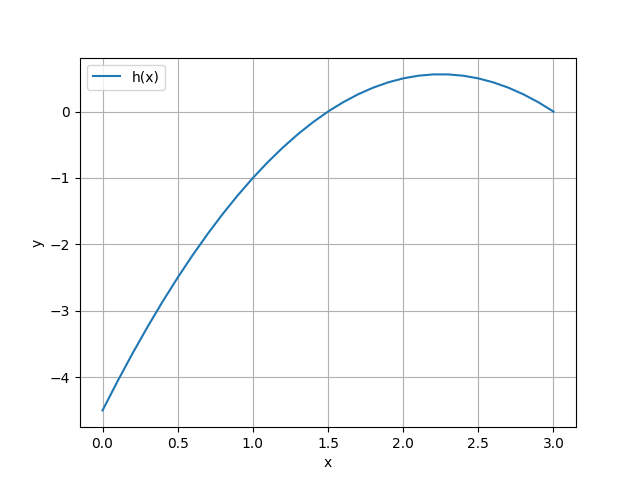
\includegraphics{Geometrie.png}
\end{center}
\begin{subparts}
\subpart Tracer le tableau de signe de $h(x)$. (Attention à l'emplacement du $0$ en ordonnée).
\subpart En déduire l'ensemble des solutions du problème.
\end{subparts}
\end{parts} 
\end{questions}
\end{document}